\documentclass[%
  % draft,
  % background,
  dvipsnames,
  svgnames,
  a4paper,
  article,
  10pt,
]{nefermemoir}

\usepackage{pgfplots, pgfplotstable}
\pgfplotsset{compat=1.12}

\usepackage{pgf,tikz}
\usetikzlibrary{%
  backgrounds,
  calc,
  math,
  shadings,
  fadings,
  patterns,
  shapes.multipart,
  arrows,
  arrows.meta,
  positioning,
  shadows,
  decorations.text,
  decorations.markings
}
\usepackage{xstring}

\newcommand{\cylindre}[4]{%
  \pgfmathsetmacro{\h}{#1}
  \pgfmathsetmacro{\L}{#2}
  \pgfmathsetmacro{\l}{#3}

  \begin{scope}[transparency group, opacity=0.85]
    \begin{scope}[fill=#4]
      \fill (-\L, 0.0) rectangle ++ (2*\L, \h) ;
      \fill ( 0.0, 0.0) circle [x radius=\L, y radius=\l] ;
      \fill ( 0.0, \h) circle [x radius=\L, y radius=\l] ;
    \end{scope}
  \end{scope}

  % bas du cylindre
  \draw [opacity=0.33, dashed]
        ( 0.0, 0.0) circle [x radius=\L, y radius=\l] ;
  \begin{scope}
    \clip ([shift={(-2pt,-2pt)}] -\L,-\l) rectangle 
          ([shift={( 2pt, 0pt)}]  \L, 0.0) ;
    \draw ( 0.0, 0.0) circle [x radius=\L, y radius=\l] ;
  \end{scope}
  % haut du cylindre
  \draw ( 0.0, \h) circle [x radius=\L, y radius=\l] ;
  % bords du cylindre
  \foreach \x in {-\L, \L} {
    \draw (\x, 0.0) -- ++ ( 0.0, \h) ;
  }
}

%======================================================================
\title{Zelliges}
\author{\SL}
\date{2000}

\hypersetup{%
  pdftitle  = {Zelliges}, 
  pdfauthor = {Sonia Labetoulle}
}
% pdfsubject % pdfcreator % pdfproducer % pdfkeywords

%======================================================================

%%%%%%%%%%%%%%%%%%%%%%%%%%%%%%%%%%%%%%%%%%%%%%%%%%%%%%%%%%%%%%%%%%%%%%%
\begin{document}

\pagestyle{empty}
% \maketitle
%%%%%%%%%%%%%%%%%%%%%%%%%%%%%%%%%%%%%%%%%%%%%%%%%%%%%%%%%%%%%%%%%%%%%%%

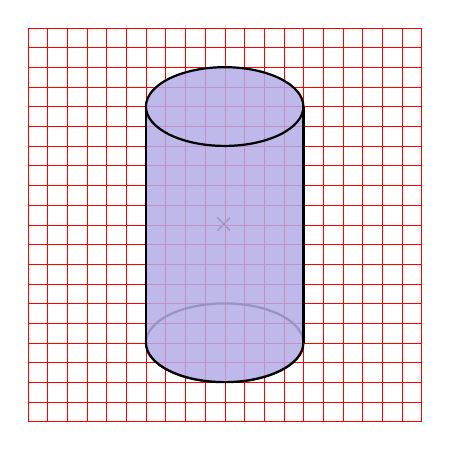
\begin{tikzpicture}[
  scale=0.5,
  % ->, 
  >=stealth',
  thick,
  % x={(-3.85mm,-3.85mm)},
  % y={(10mm,0mm)},
  % z={(0mm,10mm)},
]
  \coordinate (O) at ( 0., 0.) ;
  \node at (O) {\texttimes} ;

  \begin{scope}[help lines, ultra thin]
    \draw [step=0.5, red] (-5.,-5.) grid ( 5., 5.) ;
  \end{scope}

  \draw ( 0.0,-3.0) circle [x radius=2, y radius=1] ;
  \begin{scope}[transparency group, opacity=0.85]
    \begin{scope}[fill=SlateBlue!50!white]
      \fill ( 0.0,-3.0) circle [x radius=2, y radius=1] ;
      \fill (-2.0,-3.0) rectangle ( 2.0, 3.0) ;
      \fill ( 0.0, 3.0) circle [x radius=2, y radius=1] ;
    \end{scope}
  \end{scope}
  \begin{scope}
    \clip (-2.0,-4.0) rectangle ( 2.0,-3.0) ;
    \draw ( 0.0,-3.0) circle [x radius=2, y radius=1] ;
  \end{scope}
  \draw ( 0.0, 3.0) circle [x radius=2, y radius=1] ;
  \draw (-2.0,-3.0) -- (-2.0, 3.0) ;
  \draw ( 2.0,-3.0) -- ( 2.0, 3.0) ;
\end{tikzpicture}
%
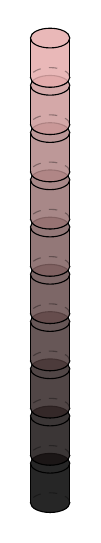
\begin{tikzpicture}[
  scale=0.5,
  >=stealth',
  thin,
]
  % \coordinate (O) at ( 0., 0.) ;
  % \node at (O) {\texttimes} ;

  % \begin{scope}[help lines, ultra thin]
  %   \draw [step=0.5, red] (-5.,-5.) grid ( 5., 5.) ;
  % \end{scope}

  % % \draw [green]
  % %       (O) circle [x radius=2, y radius=1] ;

  % \pgfmathsetmacro{\h}{3.0}
  % \pgfmathsetmacro{\L}{3.0}
  % \pgfmathsetmacro{\l}{1.0}


  % \begin{scope}[transparency group, opacity=0.85]
  %   \begin{scope}[fill=SlateBlue!50!white]
  %     \fill (-\L, 0.0) rectangle ++ (2*\L, \h) ;
  %     \fill ( 0.0, 0.0) circle [x radius=\L, y radius=\l] ;
  %     \fill ( 0.0, \h) circle [x radius=\L, y radius=\l] ;
  %   \end{scope}
  % \end{scope}

  % % bas du cylindre
  % \draw [opacity=0.33, dashed]
  %       ( 0.0, 0.0) circle [x radius=\L, y radius=\l] ;
  % \begin{scope}
  %   \clip ([shift={(-2pt,-2pt)}] -\L,-\l) rectangle 
  %         ([shift={( 2pt, 0pt)}]  \L, 0.0) ;
  %   \draw ( 0.0, 0.0) circle [x radius=\L, y radius=\l] ;
  % \end{scope}
  % % haut du cylindre
  % \draw ( 0.0, \h) circle [x radius=\L, y radius=\l] ;
  % % bords du cylindre
  % \foreach \x in {-\L, \L} {
  %   \draw (\x, 0.0) -- ++ ( 0.0, \h) ;
  % }

  \begin{scope}[yshift=0cm]
    \cylindre{1}{0.5}{0.25}{pink!00!black}
  \end{scope}
  \begin{scope}[yshift=1.2cm]
    \cylindre{1}{0.5}{0.25}{pink!10!black}
  \end{scope}
  \begin{scope}[yshift=2.4cm]
    \cylindre{1}{0.5}{0.25}{pink!20!black}
  \end{scope}
  \begin{scope}[yshift=3.6cm]
    \cylindre{1}{0.5}{0.25}{pink!30!black}
  \end{scope}
  \begin{scope}[yshift=4.8cm]
    \cylindre{1}{0.5}{0.25}{pink!40!black}
  \end{scope}
  \begin{scope}[yshift=6.0cm]
    \cylindre{1}{0.5}{0.25}{pink!50!black}
  \end{scope}
  \begin{scope}[yshift=7.2cm]
    \cylindre{1}{0.5}{0.25}{pink!60!black}
  \end{scope}
  \begin{scope}[yshift=8.4cm]
    \cylindre{1}{0.5}{0.25}{pink!70!black}
  \end{scope}
  \begin{scope}[yshift=9.6cm]
    \cylindre{1}{0.5}{0.25}{pink!80!black}
  \end{scope}
  \begin{scope}[yshift=10.8cm]
    \cylindre{1}{0.5}{0.25}{pink!90!black}
  \end{scope}

  % \draw [violet] 
  %       (-2.0, 0.0) -- ( 0.0,-1.0) -- ( 2.0, 0.0) ;

  % \draw [SlateBlue] 
  %       (-2.0, 0.0) to [out=-90, in=180]
  %       ( 0.0,-1.0) -- ( 2.0, 0.0) ;

\end{tikzpicture}

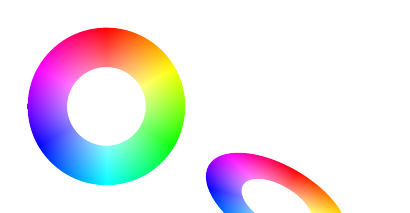
\begin{tikzpicture}
  % \fill [left color=red, right color=blue] 
  %       ( 0.0, 0.0) rectangle ( 1.0, 1.0) ;
  % \fill [left color=blue, right color=green, xshift=1cm] 
  %       ( 0.0, 0.0) rectangle ( 1.0, 1.0) ;
  % \fill [left color=green, right color=red, xshift=2cm] 
  %       ( 0.0, 0.0) rectangle ( 1.0, 1.0) ;

  % \clip 
  \shade [shading=color wheel white center, even odd rule] 
  % \fill [red, yscale=0.5] 
        ( 0.0, 0.0) circle [radius=0.5] 
        ( 0.0, 0.0) circle [radius=1] ;

  \shade [shading=color wheel white center, even odd rule, xshift=2.5cm, yscale=0.5, transform canvas={rotate=-30}] 
  % \fill [red, yscale=0.5] 
        ( 0.0, 0.0) circle [radius=0.5] 
        ( 0.0, 0.0) circle [radius=1] ;



  % \shade [shading=color wheel] 
  %       ( 0.0, 0.0) -- ++ (0:2) arc (0:36:2) -- cycle ;
  % \fill [white] 
  %       ( 0.0, 0.0) -- ++ (0:1.7) arc (0:36:1.7) -- cycle ;

\end{tikzpicture}


\def\subdivisions{10}
\begin{tikzpicture}[
  >=stealth',
  scale=5, 
  radius=2cm, 
  delta angle=30, 
]

  \begin{scope}[->]
    \draw (180:0.2) -- ( 0:2.2) ;
    \draw (-90:0.2) -- (90:2.2) ;
  \end{scope}

  \begin{scope}[draw=black]
    \filldraw [fill=red] 
              (0:0.0) -- ( 0:2.0) arc [start angle=0]  -- cycle ;
    \filldraw [fill=green] 
              (0:0.0) -- (60:2.0) arc [start angle=60] -- cycle ;
  \end{scope}

  \foreach \i [evaluate={\col=(\i+0.5)/\subdivisions*100}] in {
    0,...,\numexpr\subdivisions-1\relax
  }
    \fill [color=green!\col!red] 
          ( 0.0, 0.0) -- (\i*30/\subdivisions+30:2.00) 
          arc [start angle=\i*30/\subdivisions+30, 
               end   angle=(\i+1)*30/\subdivisions+30] -- 
          cycle ;
    \draw [line join=bevel, thick] 
          (0:0.0) -- (30:2.0) arc [start angle=30] -- cycle ;
\end{tikzpicture}


%%%%%%%%%%%%%%%%%%%%%%%%%%%%%%%%%%%%%%%%%%%%%%%%%%%%%%%%%%%%%%%%%%%%%%%
\end{document}



http://tex.stackexchange.com/questions/147852/how-can-i-shade-from-red-to-green-along-a-curve


  

A solution with a PDF shading. Problems start if you want to do this more flexible (with different angles) as there is no proper way to change the shading dependent of other values besides colors. (I tried using colors to smuggle in values but that failed already at Is there another better way to have a region with gradient opacity?)

The second example shows a simple TikZ approach by filling thirty separate slices. This is no true shading but my be enough if you need multiple different shadings. You can, of course, use more slices for better results or less slices for a faster compilation.

The actual formula for the start and end angle is:

\i*<total angle>/<number of slices>+30

and

(\i+1)*<total angle>/<number of slices>

The formula for \col is simply

\col=(\i+.5)/<number of slices>*100


\documentclass[tikz]{standalone}
\usetikzlibrary{shadings}
\makeatletter
\pgfdeclarefunctionalshading[col@ang@start,col@ang@end]{angular 30:60}
  {\pgfpointorigin}{\pgfpoint{50bp}{50bp}}{%
    \pgfshadecolortorgb{col@ang@start}\pgf@col@ang@start
    \pgfshadecolortorgb{col@ang@end}\pgf@col@ang@end}
  {exch atan 30 sub 30 div dup dup
  dup \pgf@col@ang@startred   mul exch neg 1 add \pgf@col@ang@endred   mul add
  3 1 roll
  dup \pgf@col@ang@startgreen mul exch neg 1 add \pgf@col@ang@endgreen mul add
  3 1 roll
  dup \pgf@col@ang@startblue  mul exch neg 1 add \pgf@col@ang@endblue  mul add}
\pgfset{
  angular start color/.code=\pgfutil@colorlet{col@ang@start}{#1},
  angular end color/.code=\pgfutil@colorlet{col@ang@end}{#1},
  angular start color=red,
  angular end color=green}
\makeatother
\begin{document}
\begin{tikzpicture}[scale = 5, radius=2cm, delta angle=30]
    \draw [->] (180:.2cm) -- (0:2.2cm);
    \draw [->] (-90:.2cm) -- (90:2.2cm);

    \filldraw [red,   draw = black] (0:0cm) -- ( 0:2cm) arc[start angle=0]  -- cycle;
    \filldraw [green, draw = black] (0:0cm) -- (60:2cm) arc[start angle=60] -- cycle;

    \filldraw[line join=bevel, shading=angular 30:60]
                                    (0:0cm) -- (30:2cm) arc[start angle=30] -- cycle;
\end{tikzpicture}
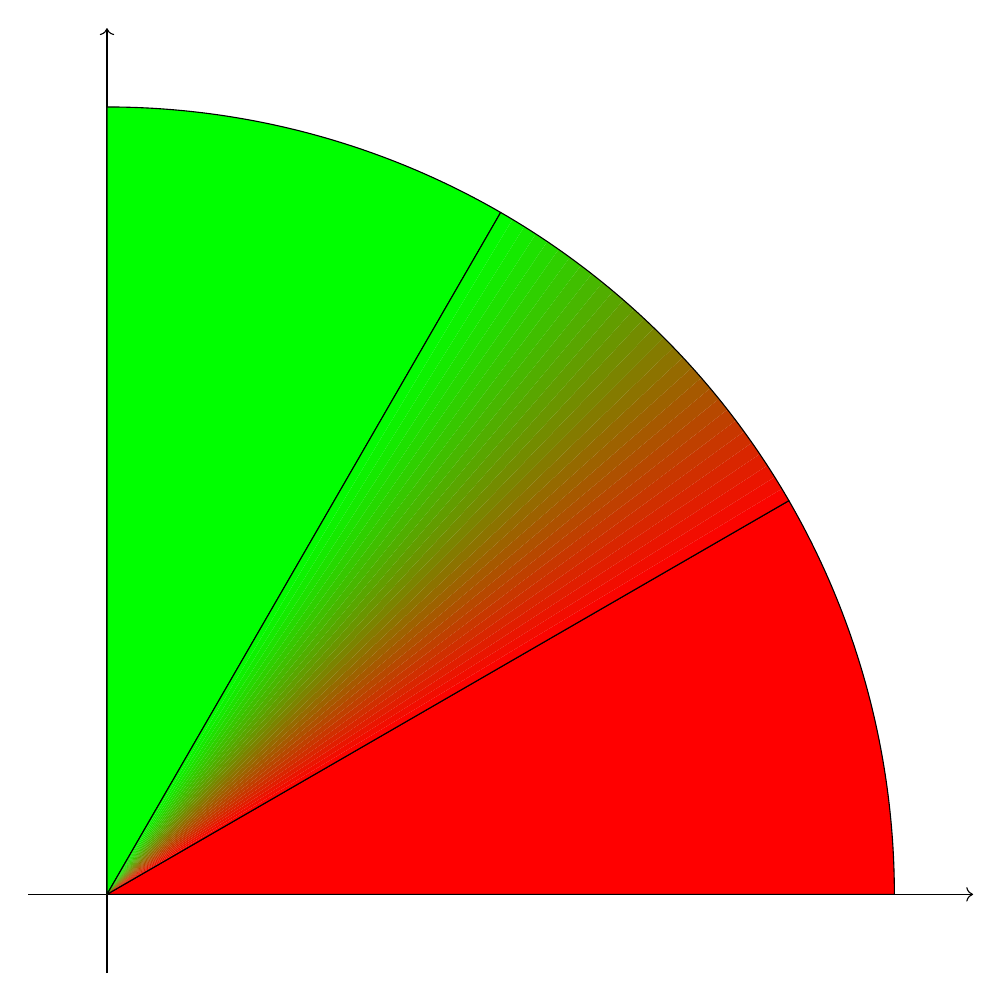
\begin{tikzpicture}[scale = 5, radius=2cm, delta angle=30]
    \draw [->] (180:.2cm) -- (0:2.2cm);
    \draw [->] (-90:.2cm) -- (90:2.2cm);

    \filldraw [red,   draw = black] (0:0cm) -- ( 0:2cm) arc[start angle=0]  -- cycle;
    \filldraw [green, draw = black] (0:0cm) -- (60:2cm) arc[start angle=60] -- cycle;

    \foreach \i[evaluate={\col=(\i+.5)/30*100}] in {0,...,29}
      \fill[color=green!\col!red]
             (0,0) -- (\i+30:2cm) arc[start angle=\i+30, end angle=\i+1+30] -- cycle;
    \draw[line join=bevel]          (0:0cm) -- (30:2cm) arc[start angle=30] -- cycle;
\end{tikzpicture}
\end{document}


Update

The code for the second picture can be made a bit more flexible:

\def\subdivisions{30}
\begin{tikzpicture}[scale = 5, radius=2cm, delta angle=30]

  \draw [->] (180:.2cm) -- (0:2.2cm);
  \draw [->] (-90:.2cm) -- (90:2.2cm);
  \filldraw [red,   draw = black] 
            (0:0cm) -- ( 0:2cm) arc [start angle=0]  -- cycle ;
  \filldraw [green, draw = black] 
            (0:0cm) -- (60:2cm) arc [start angle=60] -- cycle ;

  \foreach \i[evaluate={\col=(\i+0.5)/\subdivisions*100}] in {0,...,\numexpr\subdivisions-1\relax}
    \fill[color=green!\col!red] (0,0) -- (\i*30/\subdivisions+30:2cm) arc[start angle=\i*30/\subdivisions+30, end angle=(\i+1)*30/\subdivisions+30] -- cycle;
  \draw[line join=bevel]      (0:0cm) -- (30:2cm) arc[start angle=30] -- cycle;
\end{tikzpicture}
